\section{RepReMatch}

%\subsection{Naïve Approach}
%\begin{frame}{Naïve Approach}
%	\tikzset{
%		agent/.style = {draw, circle, font=\small, inner sep=1pt},
%		item/.style = {draw, rectangle, font=\small},
%		dots/.style = {font=\small},
%		weight/.style = {font=\footnotesize},
%		edgealw/.style = {},
%		edgeopt/.style = {},
%		edgealg/.style = {},
%		edgegry/.style = {},
%		node distance=12mm and 32mm,
%		on grid
%	}
%	\def\allocationexample{
%		\begin{tikzpicture}
%			% items
%			\node[item] (i1)                       {\(\goods_{1}\)};
%			\node[item] (i2)  [below=of i1]        {\(\goods_{2}\)};
%			\node[item] (i3)  [below=of i2]        {\(\goods_{3}\)};
%			\node[item] (im)  [below=of i3]        {\(\goods_{m}\)};
%			\node[item] (im1) [below=of im]        {\(\goods_{m+1}\)};
%			\node[dots] (id)  at ($(i3)!0.5!(im)$) {\(\vdots\)};
%			% agents
%			\node[agent] (a1) [left=of i1]  {\(\agents_1\)};
%			\node[agent] (a2) [left=of im1] {\(\agents_2\)};
%			% valuations
%			\draw[edgealg] (a1) to node[weight, pos=.42,  above]      {\(m + \epsilon\)} (i1);
%			\draw[edgealw] (a1) to node[weight, pos=.42,  above]      {\(1\)}            (i2);
%			\draw[edgealw] (a1) to node[weight, pos=.39,  above]      {\(1\)}            (i3);
%			\draw[edgealw] (a1) to node[weight, pos=.32,  above]      {\(1\)}            (im);
%			\draw[edgeopt] (a1) to node[weight, pos=.255, above]      {\(1\)}            (im1);
%
%			\draw[edgeopt] (a2) to node[weight, pos=.26,  above left] {\(m\)}            (i1);
%			\draw[edgegry] (a2) to node[weight, pos=.30,  above]      {\(0\)}            (i2);
%			\draw[edgegry] (a2) to node[weight, pos=.37,  above]      {\(0\)}            (i3);
%			\draw[edgegry] (a2) to node[weight, pos=.42,  above]      {\(0\)}            (im);
%			\draw[edgealg] (a2) to node[weight, pos=.48,  above]      {\(1\)}            (im1);
%		\end{tikzpicture}
%	}
%	\begin{columns}[c]
%		\begin{column}{.3\textwidth}
%			\(\abs{\agents} = 2\)
%
%			\(\abs{\goods} = m+1\)
%
%			\(\weight[1] = \weight[2] = 1\)
%
%			\medskip
%
%			\(\NSW(\alloc*) = \sqrt{m \cdot m}\) \\
%			\(\hphantom{\NSW(\alloc*)} = m\)
%
%			\smallskip
%
%			\(\NSW(\alloc) = \sqrt{ (2m + \epsilon - 1) \cdot 1 }\)
%			\(\hphantom{\NSW(\alloc)} \le \sqrt{2m}\)
%
%			\medskip
%
%			\(\Rightarrow \alpha \ge \sqrt{m/2} \)
%		\end{column}
%		\begin{column}{.7\textwidth}
%			\centering
%			\tikzset{
%				edgealw/.style = {thick},
%				edgeopt/.style = {thick},
%				edgealg/.style = {opacity=0.3},
%				edgegry/.style = {opacity=0.3},
%			}
%			\allocationexample
%			\hfil
%			\tikzset{
%				edgeopt/.style = {opacity=0.3},
%				edgealg/.style = {opacity=1.0, thick},
%			}
%			\allocationexample
%		\end{column}
%	\end{columns}
%	\begin{block}{}
%		What are the items of lowest valuation?\phantom{g}  % 'g' has an ascender and ensures equal margin on top and bottom.
%	\end{block}
%\end{frame}





\subsection{The Algorithm}
%\begin{frame}{Key Ideas of the Algorithm [VAR1 (if slide 6 remains)]}
%	Under submodular valuations, the set of lowest valuation is approximable only by \(\bigomega\paren[\big]{ \sqrt{m/\ln m} }\). \smash{\raisebox{-.25ex}{\Large\Lightning}}
%
%	We need change the past in three phases:
%	\begin{description}
%		\item[Phase \phasei]
%		Assign enough high-value items temporarily.
%
%		\item[Phase \phaseii]
%		Assign the remaining items definitely.
%
%		\item[Phase \phaseiii]
%		Re-assign the items of phase \phasei{} definitely.
%	\end{description}
%	\begin{center}
%		\includegraphics[height=3cm, page=43]{example-image-duck}
%	\end{center}
%	\begin{exampleblock}{}
%		A \(2n (\log_2 n + 3)\)-approximation is possible!
%	\end{exampleblock}
%\end{frame}

\begin{frame}{Key Ideas of the Algorithm}
	Naïve approach:
	\adjustfortopitem
	\begin{itemize}
		\item
		repeatedly use maximum matchings

		\item
		fails because of missing foresight
		\adjustfortopitem
		\begin{itemize}
			\item
			additive valuations:
			sort items by valuation \\
			\(\!\implies\) \(2n\)-approximation (SMatch)

			\item
			submodular valuations:
			set of lowest valuation \\
			approximable only by \(\bigomega\paren[\big]{ \sqrt{m/\ln m} }\) \smash{\raisebox{-.25ex}{\Large\Lightning}}
		\end{itemize}
	\end{itemize}
	\beamerimage at (12cm, 2cm) {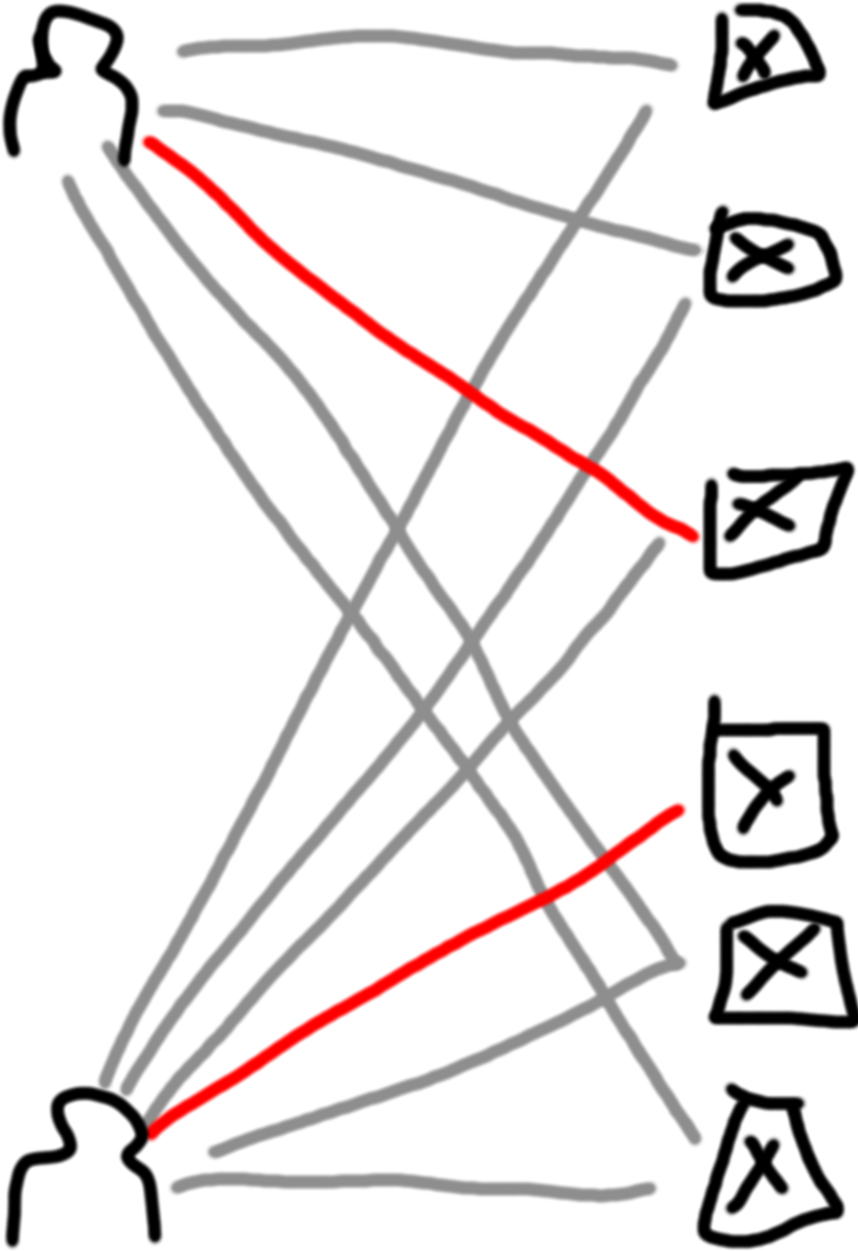
\includegraphics[height=3cm]{img/repeatedmatching}};

	\vspace{-1ex}
	We need change the past in three phases:
	\begin{description}
		\item[Phase \phasei]
		Assign enough high-value items temporarily.

		\item[Phase \phaseii]
		Assign the remaining items definitely.

		\item[Phase \phaseiii]
		Re-assign the items of phase \phasei{} definitely.
	\end{description}
	\beamerimage at (12cm, 1.25cm) {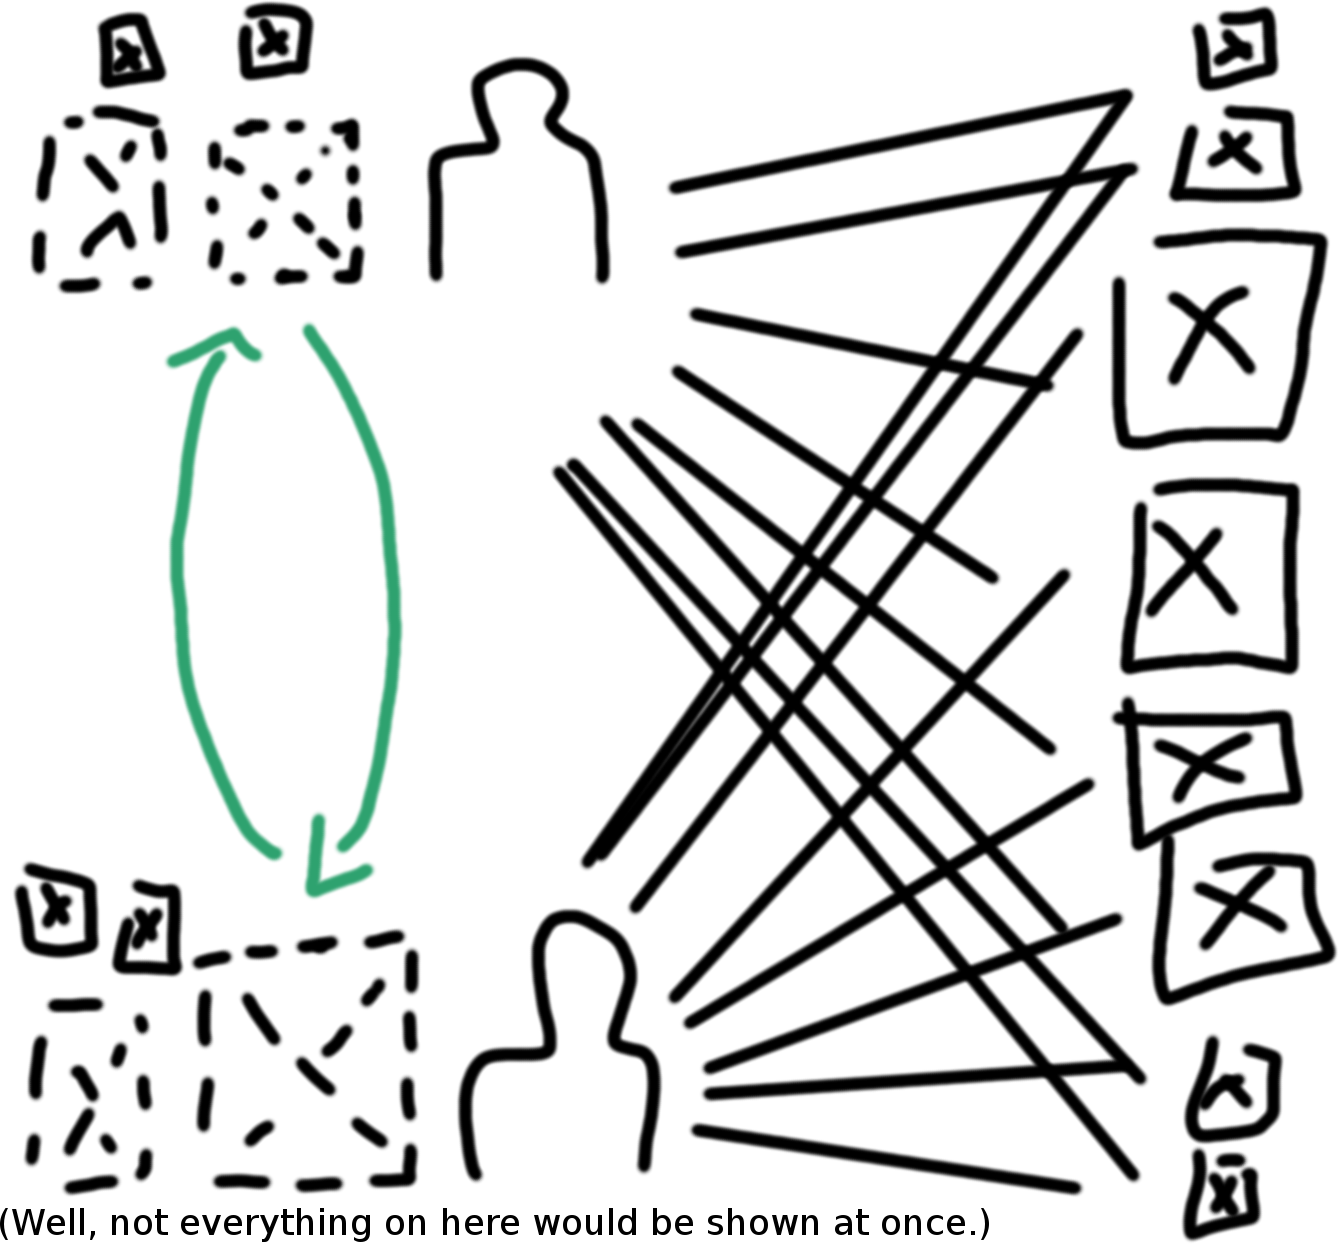
\includegraphics[height=3cm]{img/phases}};
	\vspace{0.5ex}
	\begin{minipage}{0.575\textwidth}
		\begin{exampleblock}{}
			\(\implies\) A \(2n (\log_2 n + 3)\)-approximation is possible!
		\end{exampleblock}
	\end{minipage}
\end{frame}

\begin{frame}{The Algorithm}
	Phase \phasei
	\adjustfortopitem
	\begin{enumerate}
		\item
		repeat \(\ceil{\log_2 n} + 1\) times or until \(\goods = \emptyset\)
		\begin{enumerate}
			\item
			create bipartite graph \(\bipartitegraph = (\agents, \goods, E)\) with edge weights \(\edgeweight{i, j} = \weight \log \valuations[ \hairspace j ]\)

			\item
			compute maximum weight matching \(\matching\)

			\item
			update bundles \(\alloc[\phasei]\) according to matching \(\matching\) and remove assigned items
		\end{enumerate}
		\seti
	\end{enumerate}
	Phase \phaseii
	\adjustfortopitem
	\begin{enumerate}
		\conti
		\item
		repeat until \(\goods = \emptyset\)
		\begin{enumerate}
			\item
			create bipartite graph \(\bipartitegraph = (\agents, \goods, E)\) with edge weights \(\edgeweight{i, j} = \weight \log \paren[\big]{ \valuations[\alloc[\phaseii] \cup \{ \hairspace j \} ] }\)

			\item
			compute maximum weight matching \(\matching\)

			\item
			update bundles \(\alloc[\phaseii]\) according to matching \(\matching\) and remove assigned items
		\end{enumerate}
		\seti
	\end{enumerate}
	Phase \phaseiii
	\adjustfortopitem
	\begin{enumerate}
		\conti
		\item
		create bipartite graph \(\bipartitegraph = \paren[\big]{ \agents, \bigcup_{i \in \agents} \alloc[\phasei], E }\) with edge weights \(\edgeweight{i, j} = \weight \log \paren[\big]{ \valuations[\alloc[\phaseii] \cup \{ \hairspace j \} ] }\)

		\item
		compute maximum weight matching \(\matching\)

		\item
		create bundles \(\alloc[\phaseiii]\) according to matching \(\matching\) and previous bundles \(\alloc[\phaseii]\)
	\end{enumerate}
\end{frame}





\subsection{Analysing Phases \texorpdfstring{\phasei{} \& \phaseiii}{I \& III}}
\begin{frame}{Analysing Phases \phasei{} \& \phaseiii{} (1/2)}
	Phase \phasei{} reserves \enquote{high-value} items.
	But what qualifies as \enquote{high-value}?

	\begin{definition}[14]
		Let \(\alloc* = \{ \asgd*{1}, \asgd*{2}, \dots\}\) be an optimal bundle.
		An item \(\genericitem \in \goods\) is \emph{outstanding} if \(\valuations[ \hairspace \genericitem] \ge \valuations[\asgd*{1}]\).
	\end{definition}

	\(\Rightarrow\) Are enough outstanding items reserved?
\end{frame}

\begin{frame}{Analysing Phases \phasei{} \& \phaseiii{} (2/2)}
	\adjustfortopblock
	\begin{lemma}[15]
		Each agent can be matched with an outstanding item in phase \phaseiii.
	\end{lemma}
	\begin{proof}[Sketch Proof]
		\begin{columns}[T]
			\begin{column}{0.6\textwidth}
				\begin{itemize}
					\item
					maximum number of unmatched agents halved \\
					with each round of phase \phasei
					\begin{itemize}
						\item
						\(\ceil{\log_2 n} + 1\) rounds in phase \phasei{} are enough
					\end{itemize}

					\item
					induction on number of rounds in phase \phasei
				\end{itemize}
				Base Case: In round \(1\) of phase \phasei, either
				\adjustfortopitem
				\begin{itemize}
					\item
					\(\ge n/2\) many agents matched with an outstanding item

					\item
					\(< n/2\) many agents matched with an outstanding item
					\begin{itemize}
						\item
						\(> n/2\) many items \(\asgd*{1}\) assigned to someone else

						\item
						\(> n/2\) many agents matched upon release in phase \phaseiii
					\end{itemize}
				\end{itemize}
			\end{column}
			\begin{column}{0.375\textwidth}
				\centering
				\includegraphics<1>[height=4.25cm]{img/outstanding_1}
				\includegraphics<2>[height=4.25cm]{img/outstanding_2}
				\includegraphics<3>[height=4.25cm]{img/outstanding_3}
				\includegraphics<4>[height=4.25cm]{img/outstanding_4}
			\end{column}
		\end{columns}
		\vspace{-2ex}
	\end{proof}
\end{frame}





\subsection{Analysing Phase \texorpdfstring{\phaseii}{II}}
\begin{frame}{Analysing Phase \phaseii{} (1/2)}
	\adjustforminipage
	\begin{minipage}{0.55\textwidth}
		\begin{definition}[9]
			The set \(\lostset{r}\) of \emph{lost items} is the set of all optimal items \(j \in \alloc*\) assigned to other agents \(i' \neq i\) in round \(r\).
		\end{definition}
		\begin{definition}[10]
			Let \(\alloc[\phaseii] = \{ \asgd{1}, \asgd{2}, \dots \}\) be the bundle of agent \(i\).
			The set of \emph{optimal and attainable items} is defined as
			\begin{equation*}
				\attopt{r} \coloneq \begin{cases*}
%					\alloc* \setminus \bigcup_{i' \in \agents} \alloc[\phasei][i'] & in round \(r = 0\), \\
					\alloc* \setminus \paren[\big]{ \bigcup_{i' \in \agents} \alloc[\phasei][i'] \cup \lostset{1} } & in round \(r = 1\), \\
					\attopt{r-1} \setminus ( \lostset{r} \cup \{\asgd{r-1}\} ) & in round \(r \ge 2\).
				\end{cases*}
			\end{equation*}
		\end{definition}

		\(\Rightarrow\) What is the valuation of the remaining items?
	\end{minipage}
	\beamerimage at (3.7cm, 0cm) {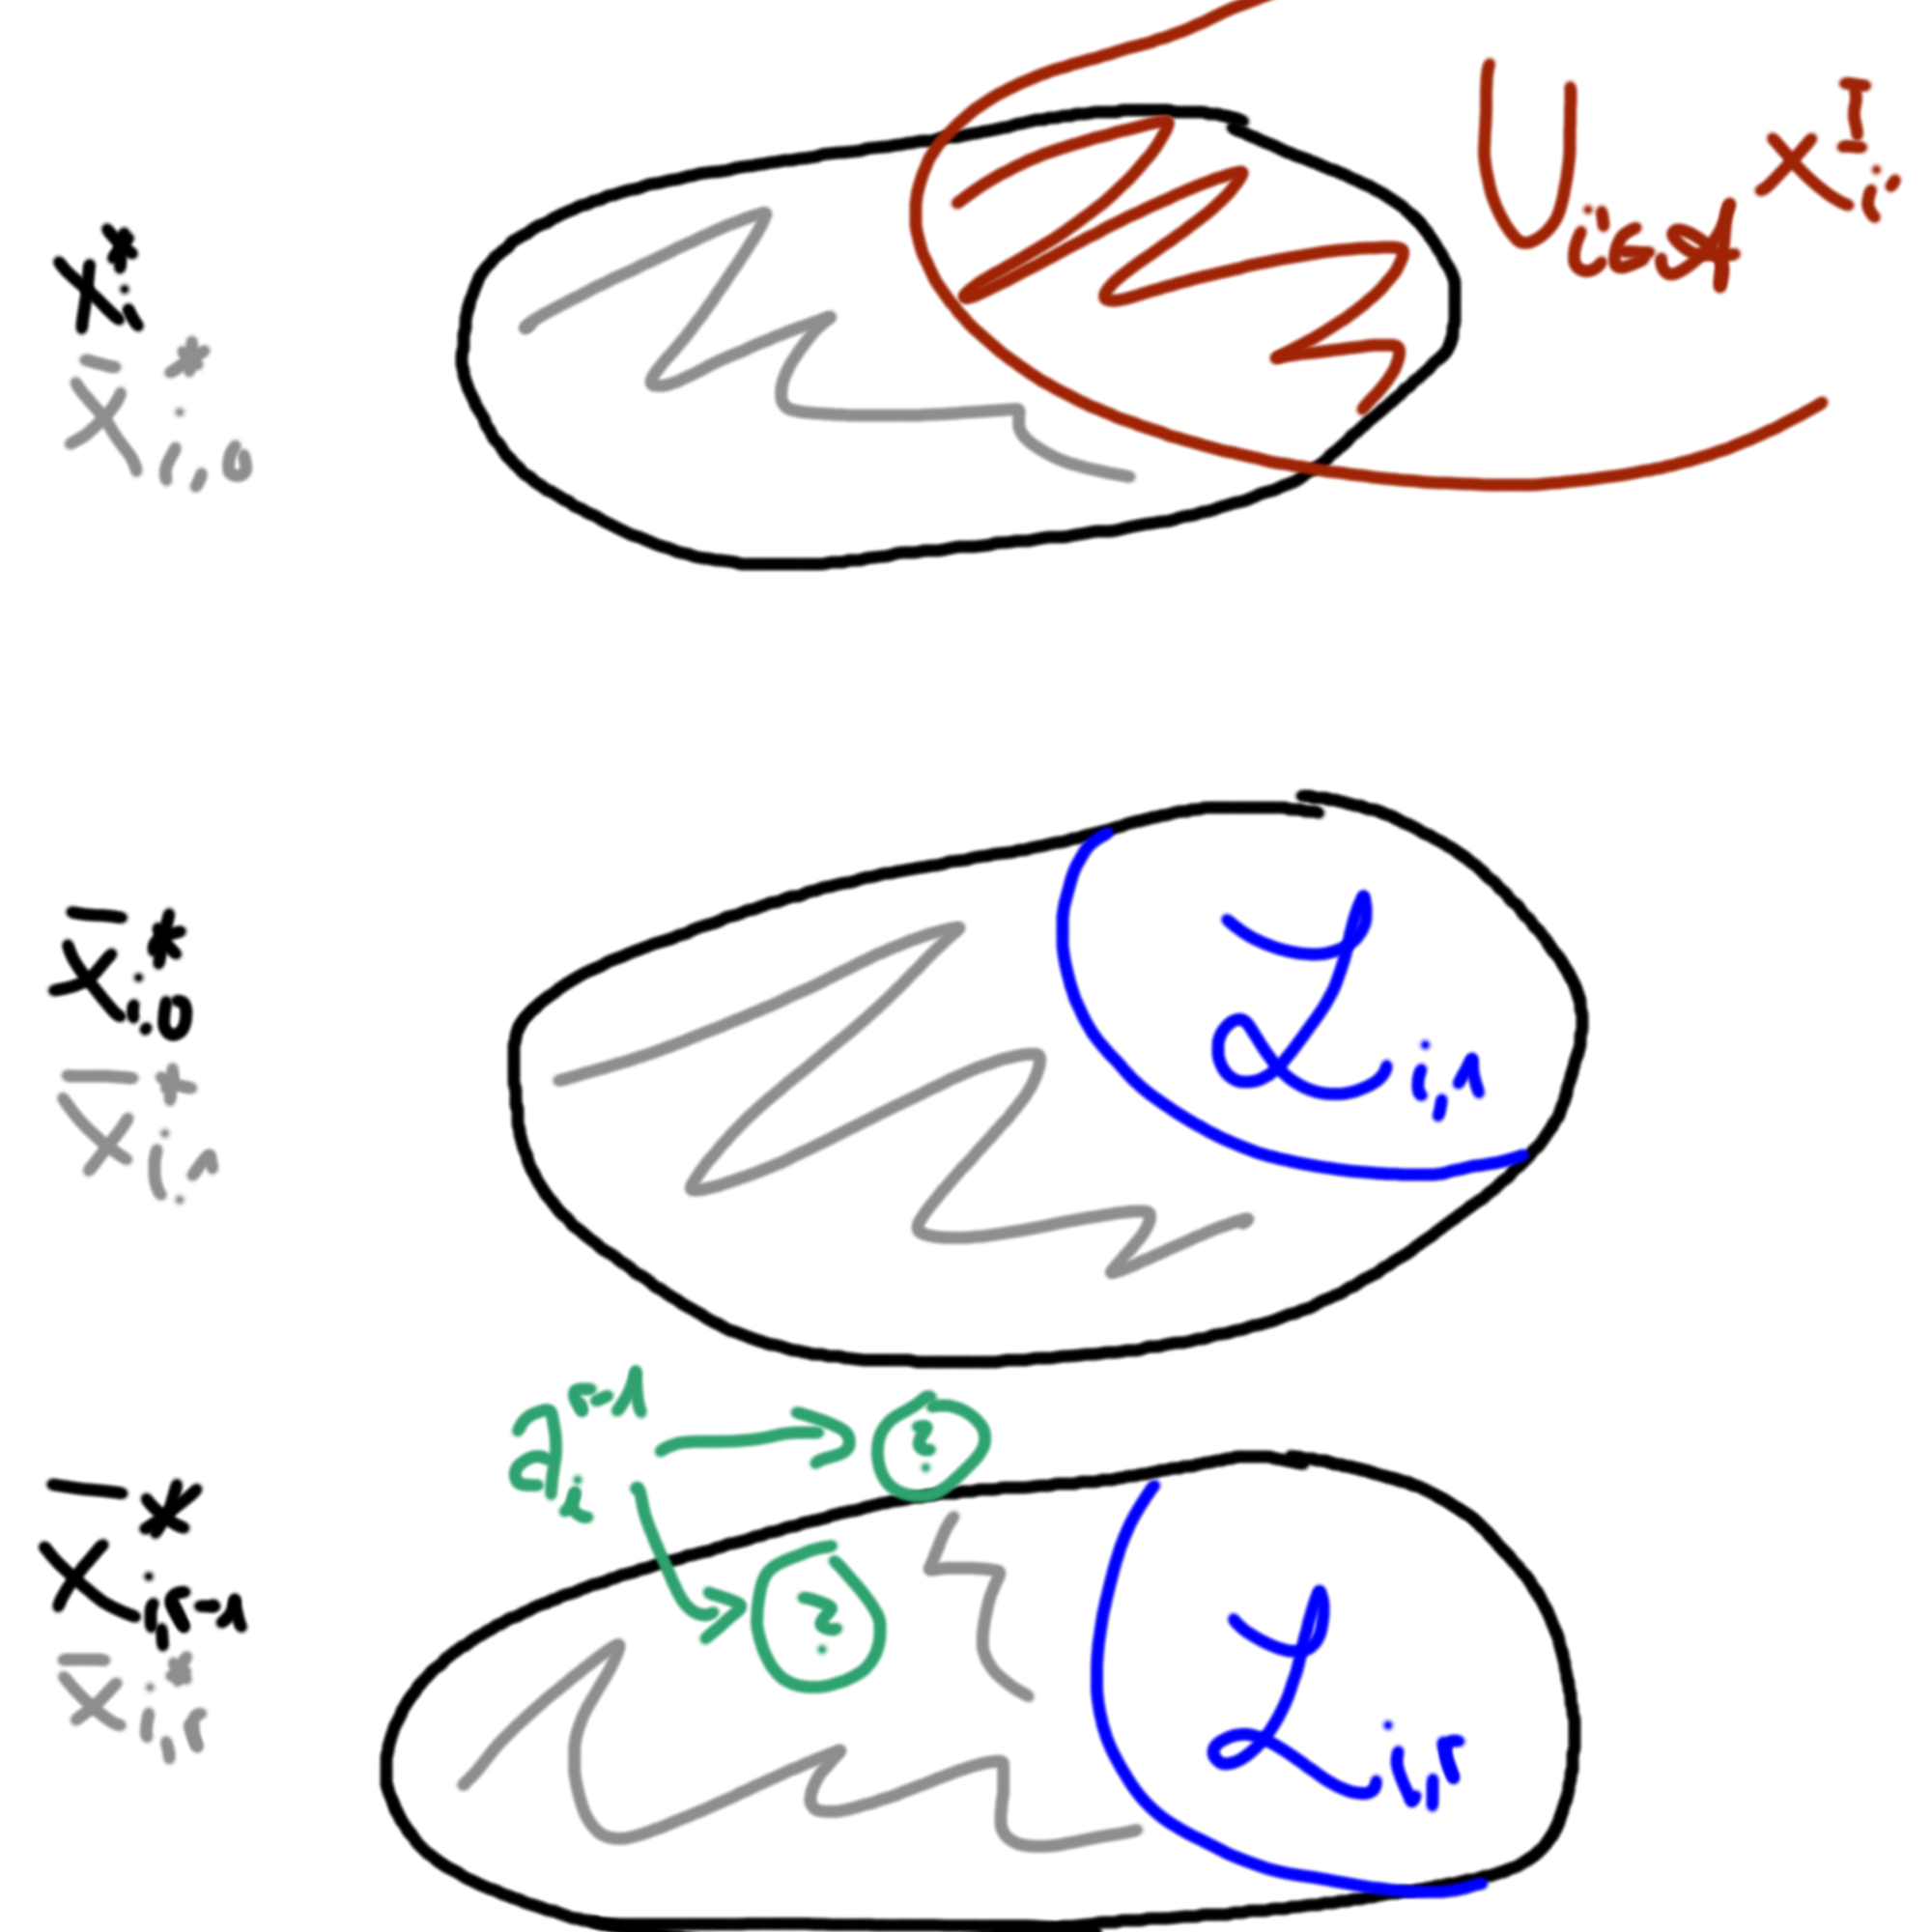
\includegraphics[width=6.5cm]{img/optainable}};
\end{frame}

\begin{frame}{Analysing Phase \phaseii{} (2/2)}
	\begin{center}
		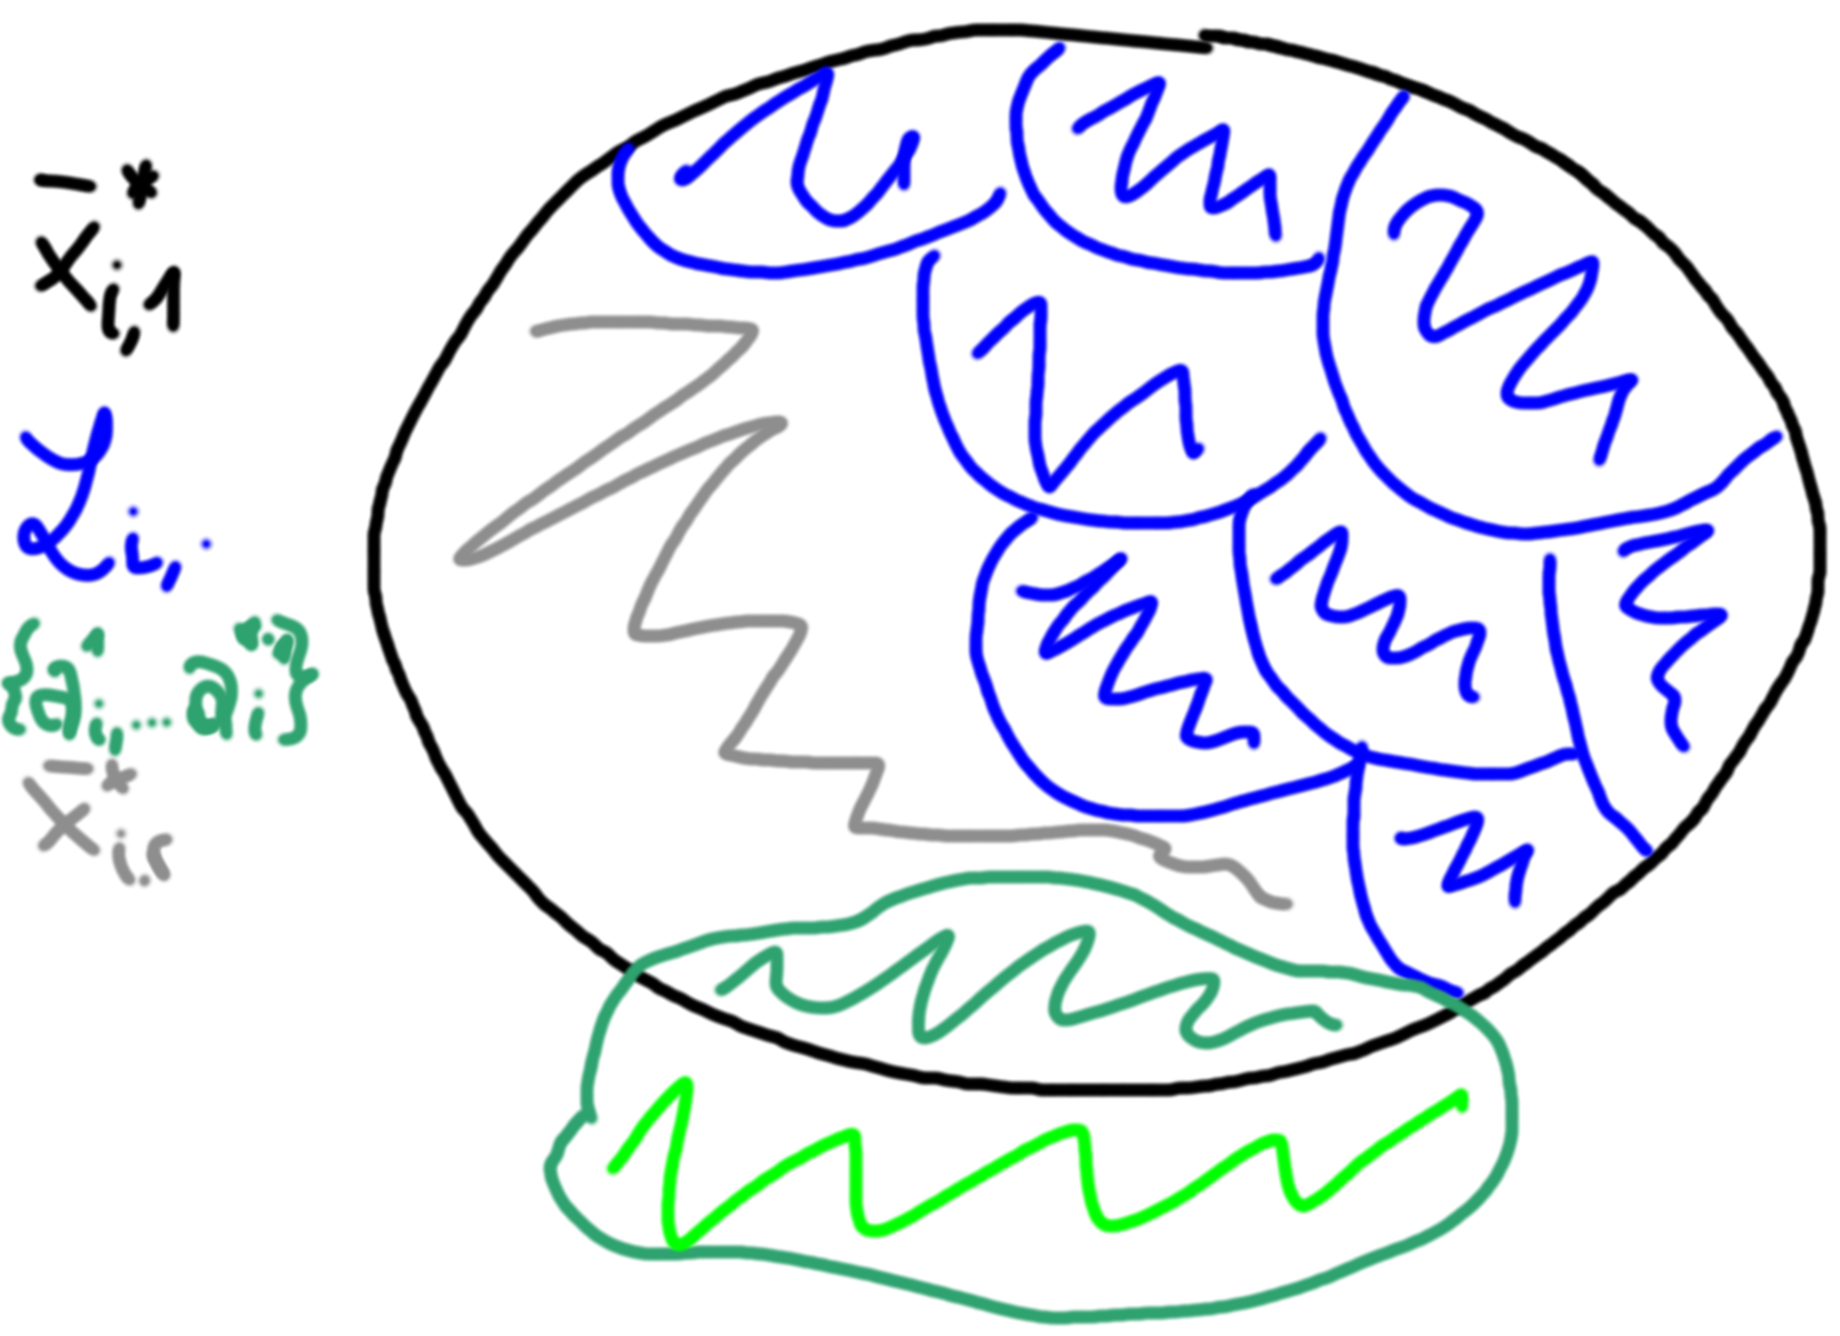
\includegraphics[height=4cm]{img/anal2_1}
		\begin{equation*}
			\valuations[ \attopt{r} \given \asgd{1}, \dots, \asgd{r-1} ]
			\ge \valuations[ \attopt{r} ] - \valuations[ \asgd{1}, \dots, \asgd{r-1} ] - \sum_{l=2}^{r} \abs{\lostset{l}} \cdot \valuations[\asgd{l-1} \given \asgd{1}, \dots, \asgd{l-2} ]
		\end{equation*}
		\scriptsize \textbf{Plan:} first show black set, then alternately enlarge green set and uncover blue sets \(\Rightarrow\) valuation of grey area = val. of black -- val. of dark green -- val. of blue \(\Rightarrow\) lower bound is enough, therefore subtract val. of whole green area \(\Rightarrow\) show that sum of marg. val. of \(\asgd{l}\) equals val. of \(\asgd{1}, \dots, \asgd{r-1}\) \(\Rightarrow\) then subtract marg. val. of blue area by summing over marg. val. of each lost set \(\Rightarrow\) marg. val. of lost set \(\le\) sum of marg. val. of items of lost set \(\Rightarrow\) marg. val. of item of lost set \(\le\) marg. val. of \(\asgd{l-1}\) because \(\asgd{l-1}\) assigned before items in lost set
	\end{center}
	\beamerimage[align=center, font=\scriptsize] at (13.5cm, 5cm) {maybe auxiliary calculation for \\ \(\valuations[ \lostset{l} \given \asgd{1}, \dots, \asgd{l-2} ]\) \\ \(= \abs{\lostset{l}} \cdot \valuations[\asgd{l-1} \given \asgd{1}, \dots, \asgd{l-2} ]\) \\ here};
\end{frame}